\subsection{Bookkeeping}
A peer will upload to and download from other peers in the network.
The peer A will want to increase its reputation and have a transaction transcribing his contribution.
A will initiate the process to create a block with peers that he has uploaded to.
These peers will be referred to as B.
This process can be seen in Figure \ref{fig:seeder-leecher}
Every block only contains one transaction.

\begin{figure}
	\centerline{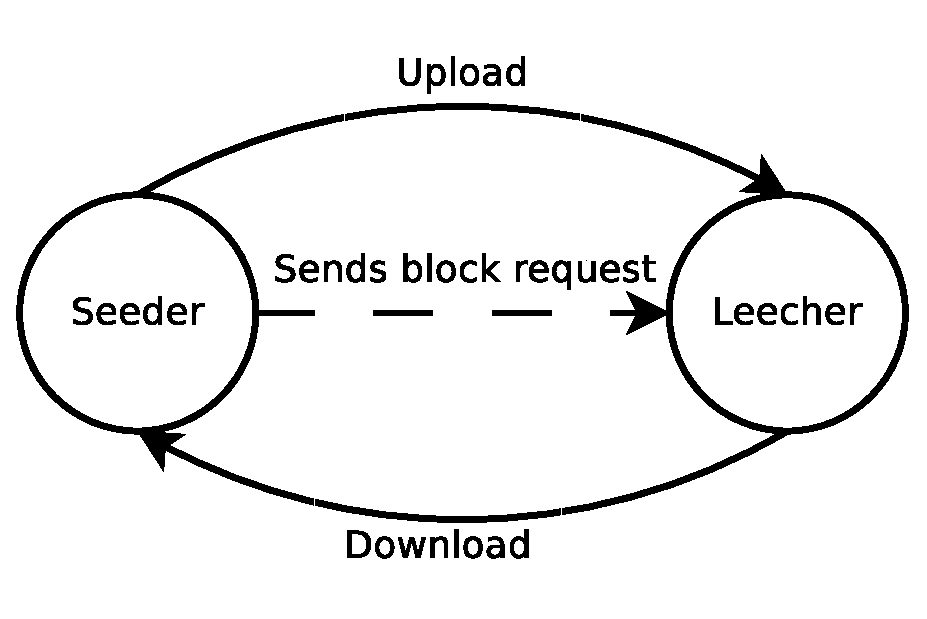
\includegraphics[scale=0.3]{design/figs/seeder-leecher.eps}}
	\caption{A seeder sending a block request.}
	\label{fig:seeder-leecher}
\end{figure}

The contents of a block can be seen in Figure \ref{fig:block}.
The up and down represents the amount that has been transferred between A and B directly for the current transaction.
Up means data uploaded by A and down the data downloaded by B.
Every peer in Dispersy has a public and private key and are unique identifiers.
A block contains both public keys of the peers,
so it is possible to verify to which peers the transaction belongs to.
The total amounts of A and B is added to the block.
This is the amount summed across the whole chain of A and B respectively.

\begin{figure}
	\centerline{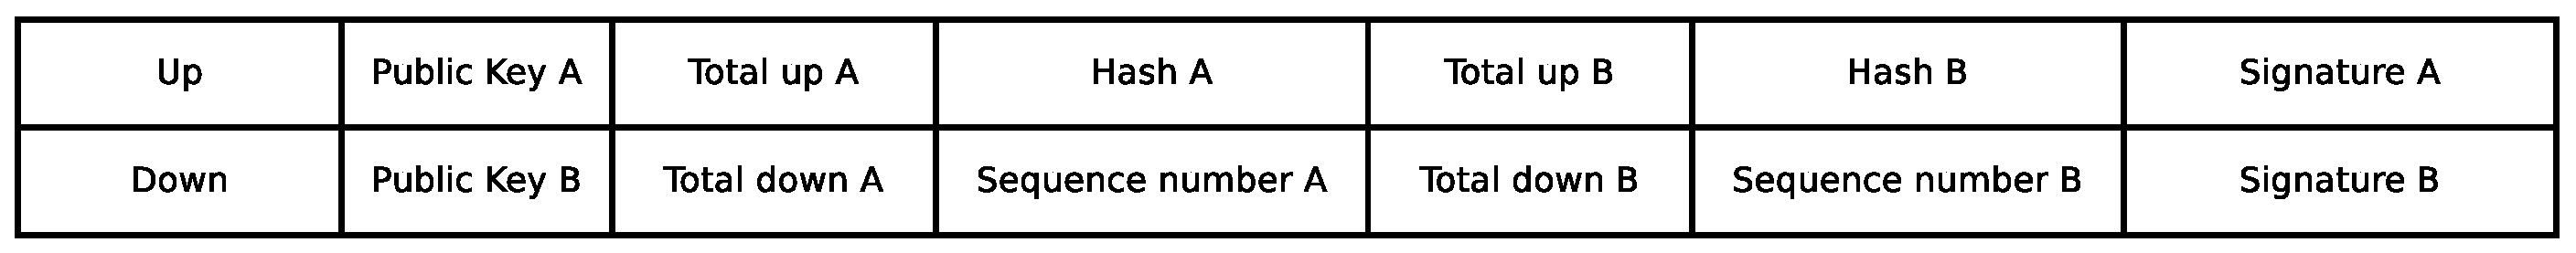
\includegraphics[scale=0.3]{design/figs/block.eps}}
	\caption{A block in MultiChain.}
	\label{fig:block}
\end{figure}

The blocks are linked to previous blocks by adding the hashes of the previous blocks of both peers.
This creates a directed acyclic graph of blocks.
An overview of a chain of blocks is seen in Figure \ref{fig:transaction-chain}.
In this overview the chain of B is currently ignored.
The first block references a special genesis hash identifying the block as the first block.
A block has two sequence numbers, one for A and for B.
These numbers allow blocks to be ordered without having to walk across the hashes linking the blocks together
Both peers add their signature to the block to announce that they approve the contents of the block.

\begin{figure}
	\centerline{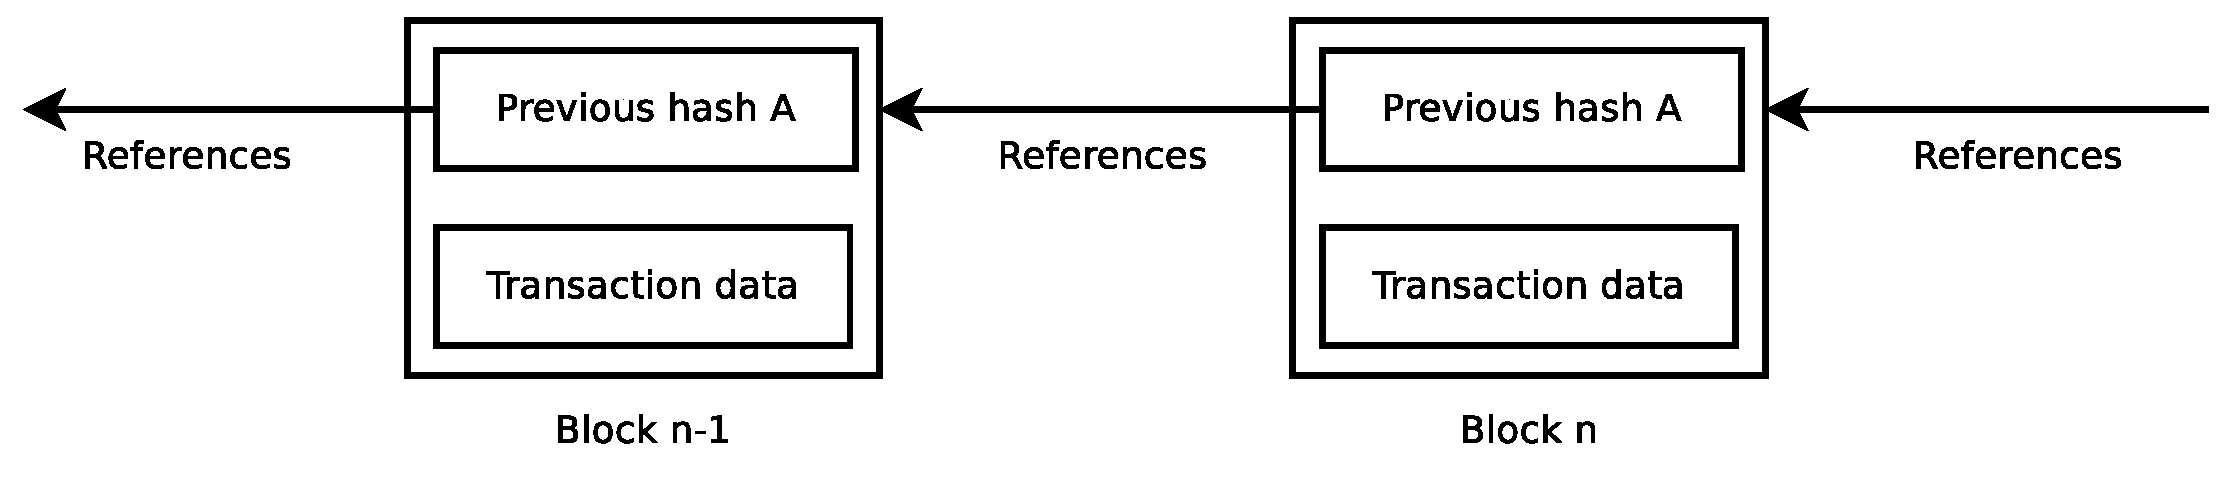
\includegraphics[scale=0.3]{design/figs/transaction-chain.eps}}
	\caption{A chain of blocks in MultiChain.}
	\label{fig:transaction-chain}
\end{figure}
